\documentclass {sig-alternate-10pt}
%\documentclass[letterpaper,twocolumn,10pt]{article}
%\documentclass{sig-alternate-10pt}
%\usepackage{usenix-2}

\input{preamble}

%\hyphenation{infra-struc-ture}
%\epstopdfsetup{outdir=./}
%\renewcommand{\baselinestretch}{0.96}

\begin{document}

\title{\retro: Enabling Low-power Duplex Visible Light Communication}
%
% You need the command \numberofauthors to handle the 'placement
% and alignment' of the authors beneath the title.
%
% For aesthetic reasons, we recommend 'three authors at a time'
% i.e. three 'name/affiliation blocks' be placed beneath the title.
%
% NOTE: You are NOT restricted in how many 'rows' of
% "name/affiliations" may appear. We just ask that you restrict
% the number of 'columns' to three.

\numberofauthors{6} %  in this sample file, there are a *total*
% of EIGHT authors. SIX appear on the 'first-page' (for formatting
% reasons) and the remaining two appear in the \additionalauthors section.

\author{
% You can go ahead and credit any number of authors here,
% e.g. one 'row of three' or two rows (consisting of one row of three
% and a second row of one, two or three).
%
% The command \alignauthor (no curly braces needed) should
% precede each author name, affiliation/snail-mail address and
% e-mail address. Additionally, tag each line of
% affiliation/address with \affaddr, and tag the
% e-mail address with \email.
%
% 1st. author
\alignauthor
Angli Liu%\titlenote{This work was conducted when Angli Liu interned with Microsoft Research Asia(MSRA)}
\\
       \affaddr{University of Washington}\\
       \email{anglil@cs.washington.edu}
\alignauthor
Jiangtao Li\\
       \affaddr{Microsoft Research, Beijing}\\
       \email{jangtao.li@gmail.com}
% 3rd. author
\alignauthor Guobin Shen\\
       \affaddr{Microsoft Research, Beijing}\\
       \email{jacky.shen@microsoft.com}
\and  % use '\and' if you need 'another row' of author names
% 4th. author
\alignauthor Chao Sun\\
       \affaddr{Microsoft Research, Beijing}\\
       \email{v-csun@microsoft.com}
% 5th. author
\alignauthor Liqun Li\\
       \affaddr{Microsoft Research, Beijing}\\
       \email{liqul@microsoft.com}
% 6th. author
\alignauthor Feng Zhao\\
       \affaddr{Microsoft Research, Beijing}\\
       \email{zhao@microsoft.com}
}


\date{25 November 2014}

\maketitle
%\pagestyle{empty}

\begin{abstract}
The new generation of LED-based illuminating infrastructures has enabled a ``dual-paradigm" where LEDs are used for both illumination and communication purposes. The ubiquity of lighting makes visible light communication (VLC) well suited for communication with mobile devices and sensor nodes in indoor environment.
Existing research on VLC has primarily been focused on advancing the performance of one-way communication. %We argue that it is essential to have bi-directional communication capability and simple combination of two one-way VLC is ill-suited for the communication between the lighting infrastructure and a mobile device.
In this paper, we present \retro, a low-power duplex VLC system that enables a mobile device to perform bi-directional communication with the illuminating LEDs over the same light carrier. The design features a retro-reflector fabric that backscatters light, an LCD shutter that modulates information bits on the backscattered light carrier, and several low-power optimization techniques. We have prototyped the \fyi{reader} system and made a few battery-free tag devices. \fyi{Experimental results show that the tag can achieve a $10kbps$ downlink speed and $0.5kbps$ uplink speed over a distance of $2.4m$. We also outline several potential applications of the proposed \retro\ system. } 

%The visible light has been used as a wireless carrier for data communication. Existing designs of Visible Light Communication (VLC) systems, however, consume significant power and only achieve one-directional communications where the mobile device is unable to transmit data to the light bulb on the same band, and hence cannot be applied to low complexity, power-constrained mobile devices or in an interactive manner without occupying extra bandwidth, extremely limiting the use of VLC in mobile and networked settings. This paper makes two main contributions: (1) we introduce the first duplex VLC system design that operates on credit card-sized battery-free devices, and (2) we introduce a communication primitive applicable to secure Radio-Frequency IDentification (RFID) systems acting against side sniffers. 
 %, and (3) we introduce a novel algorithm to detect weak and distorted signals out of strong interferences on the same spectrum that makes the system scalable
% We build a hardware prototype of the above design that can be powered solely using harvested energy from the Light-Emitting Diode (LED). The results show that our design provides benefits for VLC systems and RFID systems: it enables battery-free devices to communicate with LEDs at data rates of $10kbps$ on the downlink and $1kbps$ on the uplink and over a maximum distance of $2.2m$; it limits the uplink signal exposure area within a spindle-shaped area whose radius is less than $0.2m$. We believe that this paper represents a substantial leap in the capability and scalability of VLC systems towards previously infeasible battery-free, duplex, always and anywhere-available and secure ubiquitous communication applications.
\end{abstract}

% A category with the (minimum) three required fields
%\category{C.2.1}{Network Architecture and Design}{Wireless communication}
%A category including the fourth, optional field follows...
%\category{B.4.1}{Data Communications Devices}{Transmitters and Receivers}

%\terms{Design, Experimentation, Security}

%\keywords{Visible Light Communication, Internet of Things, Retro-reflector, RFID} % NOT required for Proceedings
%
% section by section tex files
%
\section{Introduction}
\label{sec:intro}



Nowadays, white LEDs have been prevalently deployed for illumination purpose for its advantageous properties such as high energy efficiency, long lifetime, environment friendliness, to name a few. Being semiconductor devices, LEDs also possess another feature, i.e.\, it can be turned on and off \textit{instantaneously} \cite{location3}. This effectively turns illuminating LED lights into a carrier and gives rise to a new ``dual-paradigm'' of simultaneous illumination and visible light communication (VLC). The ubiquity of illuminating infrastructure makes this dual-paradigm VLC (i.e., communication over existing lighting infrastructures) especially well suited for communication with mobile devices or sensor nodes such as streaming video to one's mobile phone or collecting environmental data from home sensors. 

Like any communication system, it is essential to have bi-directional (\ie both LED-to-device downlink and device-to-LED uplink) communication capability to ensure reliability and flexibility. For instance, a minimum requirement would be to acknowledge correct or incorrect reception of packets. %sent over the downlink (\ie LED-to-sensor), while the ability of collecting information over the uplink (\ie sensor-to-LED) from the mobile or sensor node is often highly desired. 
%Unlike existing radio communication systems where the radio front-end is shared for both transmitting and receiving, a VLC system uses an LED for transmitting and a light sensor (e.g., photodiode) for receiving. 
One immediate solution would be using another medium such as a radio link to complement the VLC link. For instance, ByteLight~\cite{ble0}, which exploits LED lighting infrastructure for both communication and localization~\cite{location1,location2}, has resorted to Bluetooth Low Energy (BLE) for the uplink device-to-LED communication. But such solution incurs additional cost and increased overall system complexity, and undermines the benefits of VLC such as security. 

In this paper, we are interested in a bi-directional communication system solely relying on VLC. An intuitive way to realize bi-directional VLC system is to put together two one-way VLC links with reverse transmitting direction, \ie a \textit{symmetric solution}. It is indeed a viable solution for dedicated VLC systems. It is perhaps a widely taken assumption, as existing work on VLC has primarily been focused on improving the throughput for one-way link using power hungry, expensive, dedicated sending/receiving devices and intermediate light concentrating optical components (\eg lenses) \cite{expensive,expensive2,retro1,retro2}. %are adopted to improve the signal to noise ratio through more directionality.  

However, the dual-paradigm nature of a VLC system and the practicality considerations render such symmetric solution not suitable, for two basic reasons. First, the dual-paradigm VLC system, with illumination being the primary goal, has quite asymmetric capabilities at the two ends: one end is the externally powered lighting LED and the other end is the power-constrained mobile or sensor device. Secondly, while the position of lights are usually fixed, that of a mobile or sensor node can be arbitrary and changing. 
%These are in sharp contrast with dedicated VLC systems where two parallel reverse direction VLC links can form a viable bi-directional solution. 
In particular, the weak end cannot afford lighting up a high power LED to transmit information especially when communicating at a relative large distance (\eg a few meters for typical indoor environments). %Even if an LED were used, the emitted light would be very unpleasant to human eyes.  
Using optical light concentrating components may allow low-power LEDs being used, but it would require precise relative positioning and careful orienting (with the optical components being steerable) between the two ends, and is obviously impractical.% This would inevitably incur much increased system complexity and cost.
%, and integrating multiple such optical components if to communicate with multiple weak nodes.  
%This is in sharp contrast with existing VLC systems where concentrating optical elements (\eg lenses) are typically used, which entail careful positioning and orientation between communicating devices. 
%Given such constraints, some early VLC-based practical systems such as ByteLight~\cite{ble0}, which exploits LED lighting infrastructure for both communication and localization~\cite{location1,location2}, have resorted to other medium, \eg Bluetooth Low Energy (BLE), for the \textit{uplink}, device-to-LED communication. This unfortunately incurs additional cost and increased system complexity. 

%Such an asymmetric setting and possibly arbitrary relative positioning of the two ends make it \textit{unfit} to compose a bi-directional communication channel using two one-way links. 
%Existing VLC work has almost unexceptionally adopted intermediate light concentrating optical components (e.g., lenses) \cite{expensive,expensive2,retro1,retro2}  to improve the signal-to-noise ratio through more directionality  While it helps to reduce the power consumption of LED, it incur much increased system complexity as it requires precise positioning of the weak nodes, the optical components being steerable, and integrating multiple such optical components if to communicate with multiple weak nodes. 

%primarily been focused on improving the throughput for one-way link using power hungry, expensive, dedicated sending/receiving devices and intermediate light concentrating optical components (e.g., lenses)  %are adopted to improve the signal to noise ratio through more directionality. 


%Also, the adoption of BLEs or LEDs for the uplink implies nearly omni-directional emissions, which accounts for extra power demand on the uplink and impose security risks as both downlink and uplink signals can be sniffed. %Finally, while some typical VLC links include intermediate optical components (e.g., lenses) to concentrate light, they lead to highly directional VLC systems and makes the actual design of a dual-paradigm VLC system deviate from the original illumination purpose. % those dedicated VLC systems aiming at extreme high data rate.}
\begin{figure}[tb!]
   \centering
   \includegraphics[width=.9\columnwidth]{system.pdf}
   \caption{System architecture.}
   \label{fig:system}
   \vskip -3mm
\end{figure}



Inspired by recent work on backscatter communication systems~\cite{abc1,abc4}, 
in this paper, we present the design and implementation of \textit{\retro} -- \textit{a low-power duplex VLC system} that consists of a reader (\reader) residing in the lighting infrastructure and tags ({\vitag}s) integrated in mobile devices or sensor nodes. The \reader is made up of an externally powered lighting LED, a light sensor (\eg photodiode) and the control circuits. The \vitag consists of a light sensor, a retro-reflective fabric, a transparent LCD shutter and the control circuits. One example tag implementation is shown in \figref{fig:system}. 

Central to \retro is the adoption of retro-reflective fabric which retrospectively reflects light, \ie bounces light back to the lighting source \textit{exactly along its incoming direction}. Its reflecting nature helps to establish an uplink over the \textit{same} visible light channel established by the high power lighting LED, which thus avoids using another high-power LED on the weak end and makes it possible to achieve the low-power design goal. %Rather, it resorts to backscattering the incoming light and communicates with the \reader over the same visible light channel. 
Its retrospective nature further not only allows arbitrary relative positioning between the lighting source and the tag, but also helps to concentrate the reflected light from a scattering light source. The two favorable properties render \retro an effective visible light based backscattering communication system. 

\retro works as follows. For the downlink (LED-to-tag), the LED in \reader switches on and off at a high frequency (\eg 1MHz, to avoid human perceptible flickering), turning the illuminating light into a communication carrier. Information bits are carried using certain modulation method (\eg Manchester coding). The light signals are picked up by the light sensor on \vitag and decoded to restore the information. 
For the uplink (tag-to-LED) communication, the same carrier is leveraged via reflection. To carry bits over the reflected light carrier, we cover the retro-reflector fabric with a transparent LCD that serves as a shutter, and adopt On-Off-Keying (OOK) modulation over the reflected light carrier by controlling the passing or blocking state of the LCD shutter.
%We further modulate the reflected light by applying an LCD as a modulator. By tuning the translucence of the LCD, we control the passing of the light reflected by the retro-reflector, and encode information bits using On-Off-Keying (OOK). 
The modulated reflected light carrier is then picked up by a photodiode on the \reader and decoded by a dedicated subsystem. 

Two major challenges arose in the design of the \retro system, especially the uplink. The root causes are the practicality considerations of the system and the low-power requirement of the tag. Specifically, the first challenge is the extremely weak and noisy signal (reflected by the remote tag) received by at the \reader. 
%When the communication range is large, the reflected light is very weak. 
We use a photodiode with wide field of view (FoV) on the \reader to avoid constraining the range of possible tag deployment. The wide FoV of the photodiode not only makes it less sensitive to the reflected lights (as only a tiny portion of its view actually corresponds to the retro-reflecting area of a tag), but also invites severe interference from the leakage and ambient reflection of the strong downlink signal and carrier.  
%The excitation of the photodiode caused by the reflected light is doomed to be small. Worse even, the wide FoV of the photodiode 
%\fyi{At the reader, the converted electrical signal is also interfered by the radio signals (\eg FM radio around 1MHz) and harmonics of the AC current. In addition, there is no clock synchronization between a \reader\ and \vitag(s).} 
Secondly, the low power consumption requirement of \vitag (in hope to achieve battery-free operation by only harvesting energy from the illuminating LED) entails careful design as well. The receiving (demodulation and decoding) unit and modulation unit (the LCD) on the \vitag consume significant energy. The LCD shutter leverages the electric field to control the arrangement of liquid crystal molecules (to polarize the light). It itself is a capacitor. Frequent charging and discharging the LCD consumes relatively significant energy, especially when the refresh rate is high. In addition, for sake of cost and energy consumption, we do not use any high precision oscillator on the \vitag. There is no clock synchronization between a \reader and \vitag(s) either.

\iffalse
\begin{figure}[tb!]
\centering
\minipage{.7\columnwidth}
      \subfigure[Front]{
        \includegraphics[width=0.45\columnwidth]{tag-front.jpg}
      } 
%      \hskip 1em
      \subfigure[Back]{
        \includegraphics[width=0.45\columnwidth]{tag-back2.jpg}
      } 
\vspace{-1ex}      
\endminipage
\caption{\vitag prototype.}
\label{fig:proto}
%\vspace{-1em}      
\end{figure}
\fi

% \begin{Itemize}
% \item Handling the high throughput LED-transmitted data is power consuming. 
% \item Transmitting with the LCD at a high toggling frequency consumes even more power than the receiver.
% \item The LED receiver must handle clock offsets from the mobile end with low clock oscillating frequency.
% \item The LED receiver has to detect retro-reflected signals 3 orders of magnitude weaker than interfering LED transmissions.  
% \end{Itemize}

%\note{liqul: put using BLE for upper-link communication into discussion.}

We have addressed these challenges with the following design. We employ a differential amplifier in the \reader receiver to filter out the noises; we adopt a multi-stage amplification design with feedbacks for automatic gain control to pull the system away from self-excitation. With these designs, we amplify the signal by up to $120dB$ while ensuring the stability of the system. We devise a sliding-window multi-symbol match filter to handle possible clock offsets and drifts between the \reader and the \vitag. To achieve low power consumption of the \vitag, we have followed the principles of using as much analog components as possible, making the circuit work at the most energy-efficient (\ie close to cut-off) state, and seeking maximal energy reuse. In particular, we avoid energy-demanding analog-to-digital converters (ADCs) with a specially designed comparator. The microcontroller (MCU) in \vitag\ handles only simple tasks such as parity check and duty cycling, and the control of LCD states. We further design an energy reuse module that collects almost half of the LCD's discharging current.

%\textbf{\retro.} To understand our \vitag\ design on battery-free ID card-sized tags, consider an LCD whose emitted light can be manipulated by an additional small circuit inside the light bulb. This circuit embeds information in the light and modulates it, while keeping the brightness of the light the same without any flickering. On the \vitag\ side, a light sensor captures the light signal that conveys information from the LED. To conserve energy, \vitag\ only uses analog components to demodulate the signal without an ADC. Upon detecting data, a low-power micro-controller on \vitag\ is waked up for uplink data transmission. It drives up the LCD to flicker, therefore sending data back to the LED by backscattering the light with a retro-reflector behind the LCD. This uplink data can be captured by a light sensor placed on the LED, along with interferences caused by downlink transmission, nearby human and object movements, household electricity fluctuations, and so on. A specifically designed receiver associated with the LED then performs the time recovery and demodulates the signal. To get a network of \vitag\/s and LEDs into play, we design a Media Access Control (MAC) protocol to mediate the communications in LEDs' illumination range. 



\fyi{We have implemented several prototypes that demonstrate the effectiveness of our \retro design. We built battery-free \vitag device, which operates by harvesting  energy from the incoming light. \figref{fig:system} depicts the architecture of a \vitag. It is the same size of a credit card, one-third of the area being the retro-reflector and two-thirds the polycrystalline silicon solar cell. We made two types of \reader, modified from a normal LED bulb and a flashlight, respectively.} 
%We also explored the tradeoff between the solar panel area and the retro-reflector area for achieving a maximum working range in the worst case where the LED is the only light source, \ie no ambient light. 

%We demonstrated the design with a battery-free credit-card-sized \textbf{\vitag}, as shown in Fig.~\ref{fig:tag}, that harvests energy of off-the-shelf LED lights. We also explored the tradeoff between the solar panel area and the retro-reflector area for achieving a maximum working range at a typical $lux$ level. 

We evaluate our system in locations where illuminating LEDs are typically deployed such as office environments. We also evaluate in dark chambers for benchmark purpose. We measure the maximum communication range between the LED and the \vitag\ with various LED illumination levels, \vitag\ orientations, solar panel areas and retro-reflector areas. Our experiments show that our $8.2cm\times 5.2cm$ \vitag\ prototype can achieve $10kbps$ downlink speed and $0.5kbps$ uplink speed over distances of up to $1.7m$ in dark chambers and $2.4m$ in offices, under a $200\mu W$ power budget. We also demonstrate its merit in security by evaluating the area around the \vitag in which uplink transmissions can be sniffed. %\fyi{Experiments show \vitag's uplink transmission cannot be detected outside of a spindle-shaped area with a $0.2m$ radius. (Jiangtao: I think we should delete this sentence)}

\paragraph{Contributions} 
We make the following contributions:
\begin{Itemize}
\item We propose a practical bi-directional VLC primitive that works for small battery-free devices using retro-reflectors and LCDs and ordinary white LEDs. The design is well suited for the communication between a mobile or sensor device and the illuminating infrastructure.
\item We address various challenges through energy-efficient analog circuit design and energy reuse components on the \vitag, and weak signal detection and unsynchronized decoding scheme on the \reader.
\item We build and evaluate real working prototypes,  confirm the effectiveness of our design and provide a sense of its practicality. %with introduction of several real application scenarios. 
\end{Itemize}
%\begin{Itemize}
%\item We present \vitag, the first visible light duplex communication system design that operates on battery-free devices while retaining a small size for them.
%\item We develop a secure communication primitive applicable to RFID systems that acts against side sniffers and malicious transmitters.
%\item Finally, we present designs and build a prototype which shows how all of the above, from \vitag, modified LEDs, through to the network stack, can be implemented on credit-card sized battery-free devices at a low cost.
%\end{Itemize}



\input{related}
\input{bg}
\section{{\bf \retro} Overview}
\label{sec:ov}


\begin{figure}[t]
   \centering
   \includegraphics[width=0.9\columnwidth]{fig/link.pdf} 
   \vskip -1ex
   \caption{Concept illustration of the \retro system.}
   \label{fig:link}
   \vskip -1em
\end{figure}


The basic design of \retro\ is to backscatter the incoming light using a retro-reflector fabric and to modulate it with an LCD. The overall concept is illustrated \figref{fig:link}. which depicts how our design support both half-duplex and full-duplex modes. %The symbol length is relatively much longer than the carrier waveform. This is due to the low refreshing rate of the commercially off-the-shelf LCDs. We want to point it out upfront that, doomed by the limited refreshing rate of LCD, our design is intrinsically asymmetric with a slow uplink.  


\subsection{Challenges}
While retro-reflecting and modulating the retro-reflected light makes it possible to establish a visible light uplink from a mobile device to the illuminating infrastructure, the actual design of \retro still faces two major challenges, rooted from the practicality and the low-power requirement of the system. 

\paragraph{Weak, Noisy Reflected Signal} 
The signal collected by the light sensor collocating at the light source is weak,  about $4$ orders of magnitude weaker than the LED emission (measured with the tag at a 1.5-meter distance and a 12W LED lamp), due to the small size of the retro-reflector and relatively large working range. 
We use a photodiode with wide field of view (FoV) on the \reader to avoid constraining the range of possible tag deployment. The wide FoV of the photodiode not only makes it less sensitive to the reflected lights (as only a tiny portion of its view actually corresponds to the retro-reflecting area of a tag), but also invites severe interference from the leakage and ambient reflection of the strong downlink signal and carrier. The converted electrical signal is further interfered by the harmonics of 50Hz (or 60Hz) AC current. 

\paragraph{Energy Efficiency} 
Secondly, the low power consumption requirement of \vitag (in hope to achieve battery-free operation by only harvesting energy from the illuminating LED) entails careful design as well. 
The receiving (demodulation and decoding) unit and modulation unit (the LCD) on the \vitag consume significant energy. The LCD shutter leverages the electric field to control the arrangement of liquid crystal molecules (to polarize the light). It itself is a capacitor. 
Frequent charging and discharging the LCD consumes relatively significant energy.
Its power consumption increases linearly with the refreshing rate. In our measurement, it consumes $84\mu A$ current at a 500Hz refreshing rate.

In addition, for sake of cost and energy consumption, we do not use any high precision oscillator on the \vitag. There is no clock synchronization between a \reader and \vitag(s) either. These consideration introduces additional challenges. 



%%There is also a derived challenge caused by our desire to further push down the energy consumption of the device. As will be elaborated in Section~\ref{sec:tagtx}, we avoided using energy expensive crystal oscillator but used a simple RC oscillator to serve as the clock. The clock generated by the RC oscillator can drift in a range of \fyi{$\pm 80\%$ from the targeted frequency}. This incurs new challenge in the decoding of the uplink signal. 


\subsection{Principles}
Inspired by design principles of some recent backscattering systems \cite{abc1,abc2, abc3}, we we apply the following design principles in addressing the challenges:
\begin{Itemize}
\item Use analog components for signal detection. This is to avoid the expensive ADC and relieve the MCU from heavy digital signal processing. 
\item Make the transistors in the circuit work at a low DC operation point (\eg close to cut-off state). This is an exploitation of the nonlinear relationship between the amplification gain and DC work current (hence energy consumption) of a triode. 
%In our amplifier design, we achieve high gain by cascading multiple low-gain amplifiers in which the triode works at almost cut-off state, instead of a single amplifier with large working current. 
%\todo{Need verification on the correctness! Need to draw the working curve of a triode?}
\item Reuse energy as much as possible. This is particularly to reduce LCD energy consumption.
\end{Itemize}


\iffalse
\begin{figure*}[t]
  \begin{center}
        \includegraphics[width=\textwidth]{../illustrations/ReadAndTag.eps}
      \vspace{-2em}
      \caption{\retro system diagram. The left part is the \reader and the right part is the \vitag. }\label{fig:sysdiagram}
  \end{center}
\end{figure*}
\else
\begin{figure}[t]
  \begin{center}
        \includegraphics[width=\columnwidth]{fig/reader_tag_simplified.pdf}
      \vspace{-2em}
      \caption{\retro system block diagram.}\label{fig:sysdiagram}
  \end{center}
\end{figure}
\fi


\subsection{Design Overview}
\figref{fig:sysdiagram} shows the architecture of a \retro system. It consists of a \reader and a \vitag. The \reader resides on the lighting infrastructure, consisting of an illumination LED and transmission logic (termed \readertx hereafter), a light sensor and the subsequent receiving circuit (\readerrx). The \vitag\ consists of a light sensor and receiving circuits (\tagrx), and a retro-reflector, a modulating LCD and other circuitry components (\tagtx).  The \readertx and \tagrx together make the \textit{downlink} visible light channel, and the \tagtx and \readerrx together make the \textit{uplink}. 
\retro operates as follows: 

\paragraph{Downlink} 
For the downlink communication, the \reader sends out information by modulating the carrier using On/Off Keying (OOK) and employing Manchester coding. This signal is captured by the light sensor of \vitag, amplified, demodulated and decoded by \tagrx in analog domain.

\paragraph{Uplink} 
As for the uplink communication, the MCU on the \vitag controls the LCD to modulate the light carrier reflected by the retro-reflector fabric. The reflected light travels back to the light sensor that collocates with the LED. Upon capture, the weak signal is first amplified with a differential amplifier to mitigate noises, further amplified, demodulated, digitized and finally decoded. Special logic has been designed to account for the possible clock drift at the \vitag when modulating the reflected carrier as we have used a cheap RC oscillator to avoid high energy cost and overly large size of crystal oscillators. 

The downlink and uplink can work concurrently on their respective bands. Hence it is capable of full-duplexing. 
Normally, when there is no traffic, the \readertx sends out the carrier by switching the LED light at a high frequency $f_0$, which should be fast enough to avoid perceivable flickering (i.e., $f_0 \gg 200$Hz). In our implementation, we set $f_0$ to $1MHz$. We support dimming of the LED by changing its DC bias. Both the receiving logic on \reader and \vitag (when turned on) keep on monitoring their own incoming light channel. With this design, a \vitag can initiate the communication to the \reader. An alternative design would be turning on the \tagtx only when \vitag\ receives certain information. This is the half-duplexing mode where only the \reader can initiate a communication session, similar to how existing RFID system works.


%In the text below, we describe our design of the \retro system in more detail. As the \readertx is of a standard design -- using an MCU to perform encoding and control the power amplifier to toggle on/off of the LED light. The concrete design choices are that we employ a 1MHz carrier,\footnote{This is a limitation from commercial off-the-shelf LED we have. If we toggle at a faster rate, the amplitude difference between On and Off state will be too small to serve as an effective carrier.} use Manchester coding and perform OOK.  We thus focus on the design of the other three components, namely \readerrx, \tagtx, and \tagrx., elaborating the key design choices.  \q{In one of the versions, we mentioned the bandwith of 100kHz. What does this number matter?}


%\input{principle_2}
\section{\retro System Design}\label{design}
In this section, we describe our design of \retro in more detail. \retro consists of a \reader and a \vitag, each of which contains the transmitting and receiving logic. We elaborate their design one by one, starting with the transmitter of the \reader. Its detailed diagram is shown in \figref{fig:diagram_reader}.

%The system consists of \readertx, \readerrx, \tagtx, and \tagrx. The first two belong to the \reader\ and the last two belong to the \vitag.  
\subsection{\readertx Design}
The \readertx employs a standard VLC design as in other work:  it performs encoding using an MCU and toggles the LED light to control the power amplifier. Specifically, we employ a 1MHz carrier and perform on-off keying (OOK) and Manchester coding. The communication bandwidth we use is 10kHz. 

Note that we may use even higher carrier frequency and larger communication bandwidth. We made the choice due to the limitation of ordinary commercial off-the-shelf LED we have. If we toggle at a faster rate, the amplitude difference between On and Off state will be too small to serve as an effective carrier. We use 10kHz bandwidth as it suffices applications we have in mind, e.g., send back the tag ID and certain sensor information it may carry.

%We next focus on the design of the other three components, elaborating on the key design choices. 


\begin{figure}[!th]
\centering
\includegraphics[width=\columnwidth]{fig/read_diagram.pdf}
\vspace{-1em}
\caption{Circuit diagram of \reader. }
\label{fig:diagram_reader}
\end{figure}

\subsection{\readerrx Design}\label{ssec:readerrx}
%\subsection{\reader Transmitter (\readertx)} \label{subsec:LEDtrans}

%As shown in Fig.~\ref{fig:sysdiagram} (b), the transmitter on \reader\ is composed of a crystal oscillator that runs at 1MHz\footnote{The fastest flickering rate of our LED is 1MHz},\remind{Later on when we say using only RC oscillator for energy savings, do we have any measurement of the energy consumption of a crystal oscillator? We need to provide the number. \hl{also the size requirement}} and an MCU followed by two amplifiers. The MCU-generated bits toggle the crystal oscillator to OOK the signal with Manchester encoding. The modulated signal will then be amplified and fed to a LED. To make sure the brightness of the LED does not pose a difference between the transmitting and not transmitting state, we add a DC component to the signal. The magnitude of the DC component is adaptable so that we can dim the brightness of the LED emission. In addition to the dimming support, flickers are avoided in \reader\ transmitter. We use 10kHz as the symbol rate, which far exceeds the frequency (200 Hz) below which human eyes will feel of fluctuations, which could disturbing and unacceptable. 

% We illustrate a typical packet the LED transmits in Fig.~\ref{fig:commdiagram}.

% \begin{figure}[!t]
% \vskip -0.03in
%   \centering
%       {
%         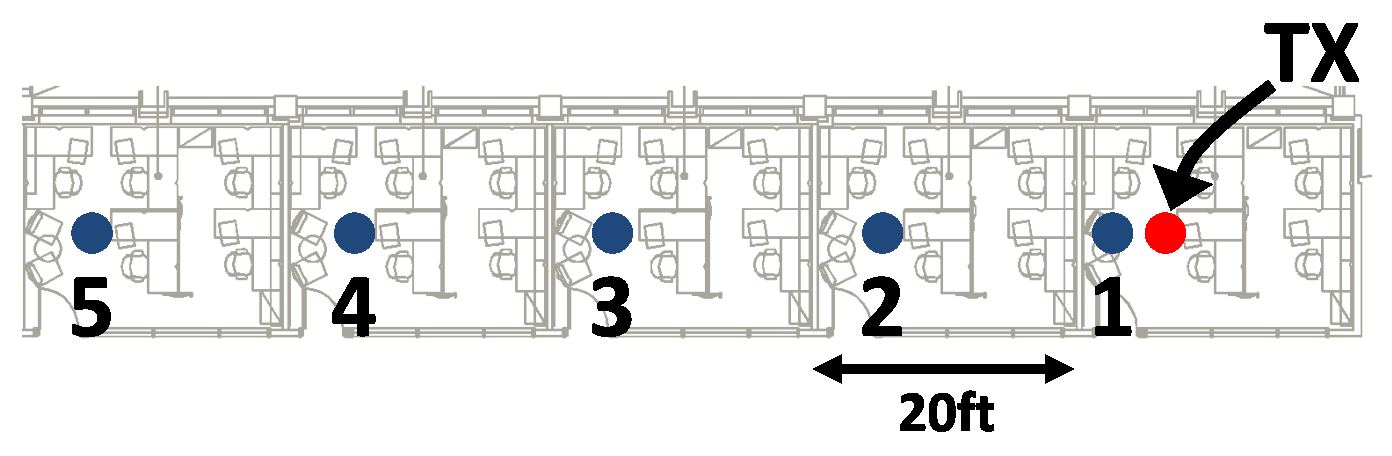
\epsfig{file=../figures/layout2.eps, width=0.6\columnwidth}
%       }
% \caption{{\bf An LED-transmitted Packet} \hl{blah}.}
% \label{fig:commdiagram}
% \vskip -0.05in
% \end{figure}

%\subsubsection{Challenges of \readerrx Design}
%\paragraph{Challenges of \readerrx Design}
The major challenges that arise in the design of the \readerrx are the following. First of all, the signal from the \vitag reflection is extremely weak, especially due to the use of the small retro-reflector on the \vitag. Second, the signal is severely interfered by other light and electrical sources. In particular, as the light sensor sits next to the LED, it is likely that there is leakage from downlink signals and carrier, in additional to the diffusing reflections from the ambient sources. Because of the close distance, the interference is several orders of magnitude greater than the actual reflected signal from the \vitag. As measured \fyi{in one implementation of 12W LED lamp}, the power of the \vitag-reflected signal is about $-80dBm$ \fyi{at 1.5 meters} while the \readertx emitted light signal can be up to $30dBm$. In fact, these interference could cause the \readerrx amplifiers to saturate without careful design. In practice, the light reflected by the movement of humans and other objects around also causes such interference. 
Thirdly, the converted electrical signal is also interfered by commercial FM radios that operate around 1MHz. The harmonics of the $50-60$Hz AC supply of the lighting infrastructure also matters, which is on par with the toggling rate (0.5kHz) of our LCD modulator. %The harmonics be relatively strong than the reflected signal.
%\remind{We may move this AC harmonics to the part explaining the performance differences between indoor and outdoor, as we do not have special treatment of this noise source. or do we???}
Last but not the least, our choice of using a small and low frequency RC oscillator at the \vitag, instead of high-precision oscillator (for sake of energy consumption reduction), makes the reflected signal suffer from clock offsets and drifts.   


In our design, we first try to isolate the receiving path, both the circuit and light sensor, from the transmitting path. In practice, we use 4-layer PCB and always ensure the wires are covered by two copper layers connected to ground. We also shield the light sensor to avoid leakage of the downlink signals. 

In the rest of this section, we elaborate the modular and algorithmic designs of \readerrx that overcome these challenges.  


%\subsubsection{Amplification and Demodulation}
%Since the received signal is extremely weak (the order of uV), we apply four successive RF amplifiers (gain>80dB), an active detector with a high-speed operational amplifier (gain=0dB) and a baseband amplifier (gain=100dB) to achieve superior total performance (gain>100dB). The detailed design is the following. 
\paragraph{Amplification and Demodulation}
As shown in \figref{fig:diag-reader}, an external light sensor with a parallel inductor captures the \vitag signal and performs preliminary band-pass filtering. The photocurrent is then amplified by a subsequent preamplifier and further transmitted to the internal (\ie on the \reader board hosted within the lamp) amplifier and processing circuit. An impedance matching module is incorporated. 

The pair of transmission lines is relatively long, decoupling the front end and the subsequent processing unit.%and easily interferes with \textit{common-mode noises} such as the radio and AC harmonics. 
As the two wires are equally affected by the common-mode noises, we thus design a tuned differential amplifier as the first-stage internal amplifier. By subtracting the signals from the two wire, the differential amplifier effectively eliminates the common-mode noises. It further suppresses other off-band noises through LC resonance at 1MHz carrier frequency. As the reflected signal from \vitag\ is extremely weak, we further amplify it through two additional LC-structured amplifiers. The overall amplification gain is $80dB$. 
This signal then goes through a high precision envelope detector to pick up the baseband signal from the carrier. 
%, which realizes regular passive diode demodulation that picks out the baseband signal from the $1MHz$ carrier but with much lower distortions. 
Finally, the baseband signal is amplified and fed to the MCU, which performs analog-to-digital conversion and decoding therein. 

Note that the gain of the differential amplifier is programmable and controlled by the micro-controller. We also use two-stage amplifiers (instead of one-stage amplifier with very large gain) both with feedback mechanisms. These mechanisms helps pull the circuit state away from self-excitation. 


%\begin{figure*}[!t]
%\vskip -0.1in
%\centering
%{\footnotesize
%\begin{tabular}{ccccc}
%\epsfig{file=../illustrations/waveform1.eps, width=0.2\columnwidth} & \epsfig{file=../illustrations/waveform2.eps, width=0.2\columnwidth} & \epsfig{file=../illustrations/waveform3.eps, width=0.2\columnwidth} & \epsfig{file=../illustrations/waveform4.eps, width=0.2\columnwidth} & \epsfig{file=../illustrations/waveform5.eps, width=0.2\columnwidth}\\
%{(a) Normal} & {(b) Up-truncated} & {(c) Down-truncated} & {(d) Up and Down-truncated} & {(e) Average-drifted}\\
%\end{tabular}
%}
% \vskip -0.1in
%\vspace{1em}
%\caption{\footnotesize{\bf Varying Wave patterns.} Blah Blah.}
%\label{fig:dynamicRange}
%\vspace{-1em}
%\end{figure*}
%

%\begin{figure*}[!t]
%\centering
%{\small
%\begin{tabular}{cccc}
%\epsfig{file=../illustrations/waveform1.eps, width=0.22\columnwidth} & 
%\epsfig{file=../illustrations/waveform2.eps, width=0.22\columnwidth} & 
%\epsfig{file=../illustrations/waveform3.eps, width=0.22\columnwidth} & 
%\epsfig{file=../illustrations/waveform5.eps, width=0.22\columnwidth}\\
%{(a) Normal} & {(b) Top-truncated} & {(c) Bottom-truncated} & {(d) Average-drifted}\\
%\end{tabular}
%}
% \vskip -0.1in
%\vspace{1em}
%\caption{Possible Waveform patterns after baseband amplifier of \readerrx. \todo{Verify!! Is it from after baseband amp?}}
%\label{fig:dynamicRange}
%\vspace{-1em}
%\end{figure*}


\begin{figure}[!th]
  \begin{center}
      \subfigure[Normal]{
        \includegraphics[width=0.45\columnwidth]{../illustrations/waveform1.eps}\label{fig:waveform1}
      } 
      \hfill
      \subfigure[Top-truncated]{
        \includegraphics[width=0.45\columnwidth]{../illustrations/waveform2.eps}\label{fig:waveform2}
      } \\ \vspace{-1em}
      \subfigure[Bottom-truncated]{
        \includegraphics[width=0.45\columnwidth]{../illustrations/waveform3.eps}\label{fig:waveform3}
      } 
      \hfill
	  \subfigure[Average-drifted]{
        \includegraphics[width=0.45\columnwidth]{../illustrations/waveform5.eps}\label{fig:waveform5}
      } 
\vspace{-1em}
      \caption{Possible waveform patterns after the baseband amplifier of \readerrx. }\label{fig:dynamicRange}
  \end{center}
\vspace{-1em}
\end{figure}

%\subsubsection{Decoding and Handling Clock Drift}\label{subsubsec:clockoffset}
\paragraph{Decoding and Handling Clock Drift}
The clock offset and drift caused by the RC-clock of the \vitag bring challenges as we try to extract the timing information from the signal and perform the decoding at the same time. %First, we describe why common decoding methods do not work in our case.
There are several common decoding methods. One method is based on peak (or edge) detection. Its principle is to extract the extreme (discontinuous) points in the signal to detect clock beats. A second approach is averaging-based algorithm in which signal samples are averaged to generate a threshold, and samples above this threshold denote ones and below denote zeros. A third approach is symbol-based match filter that tries to match the waveform of one symbol and detects the convolution peaks to determine the accurate timing.

\begin{figure}[tb!]
\centering
\includegraphics[width=\columnwidth]{../figures/slidingWindow.eps}
\vskip -0.05in
\caption{All possible 3-bit patterns (left) and illustration of their actual voltage levels (middle), and corresponding matching templates (right) for edge detection. 
}
\label{fig:swmsmf}
\end{figure}


However, none of these methods work for us. 
Take for example the normal signal input waveform shown in \figref{fig:dynamicRange}(a). 
Due to the possible lag of the automatic gain control at the \readerrx, the high dynamic range of interference, we may obtain top- or bottom-truncated waveforms, as shown in \figref{fig:dynamicRange}(b) and (c), or both top- and bottom-truncated waveform (not shown due to space limit). Such situation would fail peak/edge detection algorithms. Similarly, the ambient brightness changes (e.g., caused by human body reflection) will likely cause a time-varying shift in average value, as shown in \figref{fig:dynamicRange}(d). This would fail the averaging-based approach. Furthermore, due to Manchester coding, one bit contains two chips -- a high volt chip followed by a low volt chip, or vice versa, indicating a `0' and `1', respectively. Other than an all `0' or all `1' sequence, the rising edge and the falling edge are not evenly spaced in time. %The correlation peak for such unevenly spaced chips will be skewed. 
%A typical example is three chips that contain one high-volt chip followed by two low-volt chips, in which case the correlation peak will be skewed, compared to the case where the voltage is high for one chip and low for the next. 
This results in two (and at most two) consecutive low (or high) voltage chips for bit sequence `01' (or `10'). 
A low voltage chip corresponds to the LCD discharging phase at the \vitag; Consecutive low chips thus correspond to continuous discharging of the LCD. As a result, the second low chip will have a lower voltage than the first one. Similarly, the second high chip will have a higher voltage than the first one in two consecutive high voltage chips. The consecutive low or high voltage chips and their corresponding voltage level are depicted in \figref{fig:swmsmf}. 
In the face of these distortions, the single-symbol match filter method will fail, because the correlation peak will be skewed for those unevenly spaced high/low voltage chips.

%\vskip 0.05in\noindent{\bf \hl{CDMA-based algorithms}} use a string of chips to represent one bit~\cite{abc1}, and does correlation on the receiver side to decode the bit by finding the peak of the correlation result. The algorithm can pinpoint the clock and hence decode the signal in a low SNR situation, but it is not suitable for low symbol-rate channels like the uplink in our case. 

%\vskip 0.05in\noindent{\bf One-symbol \qm{match filter} algorithms} try to match the wave form of the signal and detects the convolution peaks to determine the accurate timing. However, due to the rough equivalence of the LCD on the tag side that shapes a bit and a capacitor, the basic wave form tends to be sawtooth, as shown in Fig.~\ref{fig:dynamicRange} (a) when there is no top or bottom truncation. Further, as the bits are encoded in Manchester code, the rising edge and the falling edge are not necessarily symmetric in time. A typical example is three chips that contain one high-volt chip followed by two low-volt chips, in which case the correlation peak will be skewed, compared to the case where the voltage is high for one chip and low for the next. Therefore, the timing will be biased.


%\noindent\textbf{\textit{Sliding-window Multi-symbol Match Filter:  }}
We develop a novel algorithm, termed \textit{sliding-window multi-symbol match filter} algorithm, to decode the signals from Manchester coding that subject to a huge dynamic range. %The approach extends the one-symbol match filter to that with an addition regarding clock adjustment using a multi-symbol match filter. 
The basic idea is to avoid the biased timing caused by skewed correlation peaks in the conventional symbol-based match filter method, by matching \textit{all possible patterns} of the waveform that may result from Manchester encoding, and iteratively adjusting the local clock by every bit period. To begin with, the algorithm exploits standard correlation to detect the preamble of a packet. In our design, preambles last for a time period equivalent to 3 Manchester chips.
%\fyi{Preambles are a string of eight `1's in our design. Its chips are evenly distributed and alternating between high and low voltages, and hence can be accurately detected}
%, using the fact that the preamble is different from any possible bit patterns in the payload and is known beforehand. 
Upon finding the preamble, the algorithm estimates the length of a bit using the knowledge of the \vitag clock which is known but subject to offsets and drifting. Then the algorithm iteratively performs the following two steps:
\\[4pt]
\noindent\textit{Step 1: Template Matching.} For all the samples within the three-bit span, we match them against the corresponding template, as shown in \figref{fig:swmsmf}. Note that the template is of amplitude of $\pm1$, so as to most precisely detect the rising or falling edges of the bit in the middle. Ideally, the right correlation yields a peak in the middle of the three bits. 
\\[4pt]
\noindent\textit{Step 2: Local Time Recovery.} 
%Then the algorithm adjusts the clock estimation by correlating the three bits from the raw signal against the corresponding gold pattern from the eight patterns. 
Due to the time variance with the start of the packet and the frequency deviation between the clocks of the \reader and the \vitag, the peak correlation does not necessarily align with the actual timing of the edge. This yields errors in clock estimation. To bound this error as the decoding goes, we perform linear regression $t=k\cdot s+s_0$ to estimate the central time of every three bits, where $s_0$ is the initial time estimate after preamble detection, $s$ and $t$ are the central time from the \reader's view and from the \vitag's view, respectively, and $k$ denotes the clock sampling ratio of the \vitag\ over \reader. Every round $k$ is re-estimated, and then the algorithm moves the three-bit window one bit forward.
 
The whole procedure is repeated till reaching the end of the packet. This time recovery algorithm bounds the error on $t$ from diverging as the decoding process proceeds. %\todo{The proof does bounds $k$. Original text say prevent $k$ from propagating, which is not correct. How about simply put "This time recovery algorithm bounds the estimation error as the decoding proceeds."? Chao: yes, this is more appropriate} 
We formally describe this in the following lemma, for which we give a proof in Appendix.
\begin{lemma}
The time recovery algorithm ensures the error of the \vitag clock estimation to converge to zero asymptotically if a packet contains infinite number of bits. 
\label{lem:lemma1}
\end{lemma}

%Note that we choose a three-bit time span as a correlation unit because three bits are the smallest number of bits that contain all possible wave forms when the signal is Manchester-encoded. The use of three-bit window can maximize the correct detection of the bit in the middle. 


% \begin{figure}[!t]
% \vskip -0.03in
%   \centering
%       {
%         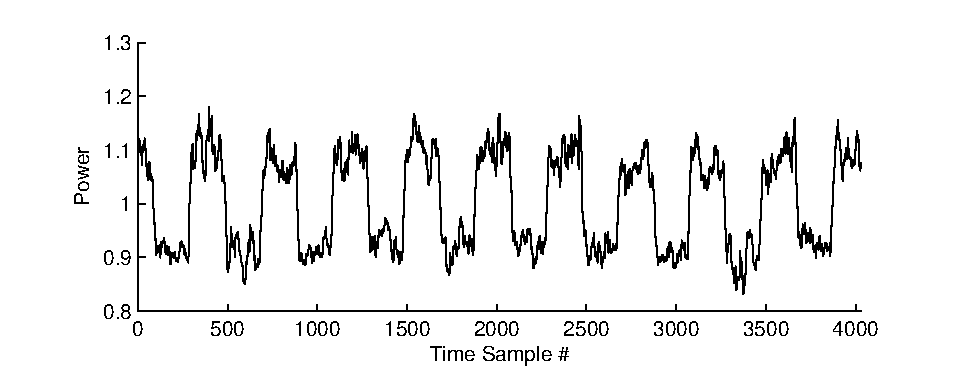
\epsfig{file=../figures/divide.eps, width=0.6\columnwidth}
%       }
% \caption{{\bf Signal Captured by the LED Light Sensor \hl{replace with a system block diagram!!}} \hl{integrates both mmm in a single design. It can operate using both RFID and TV transmissions}.}
% \label{fig:capture}
% \vskip -0.05in
% \end{figure}




%\begin{figure}[!th]
%  \begin{center}
%      \subfigure[Waveform of TP1]{
%        \includegraphics[width=0.4\columnwidth]{../illustrations/waveform_a1.eps}\label{fig:waveformOfTag_Lightsensor}
%      } 
%      \hfill
%%      \subfigure[Waveform of TP2]{
%%        \includegraphics[width=0.45\columnwidth]{../illustrations/waveform_a2.eps}\label{fig:waveformOfTag_Amp}
%%      } \\
%      \subfigure[Waveform of TP3]{
%        \includegraphics[width=0.4\columnwidth]{../illustrations/waveform_a3.eps}\label{fig:waveformOfTag_TunedAmp}
%      } 
%      \\
%	  \subfigure[Waveform of TP4]{
%        \includegraphics[width=0.4\columnwidth]{../illustrations/waveform_a4.eps}\label{fig:waveformOfTag_Dmodulator}
%      } 
%      \hfill    
%	  \subfigure[Waveform of TP5]{
%        \includegraphics[width=0.4\columnwidth]{../illustrations/waveform_a5.png}\label{fig:waveformOfTag_Thresholding}
%      } 
%
%%      \vspace{-1em}
%      \caption{Waveforms at various stages in the \tagrx. \todo{Pay attention to the units/scale. e.g., seems there is no much amplification from (a) to (b).}}\label{fig:waveformOfTag}
%  \end{center}
%%  \vspace{-0.3in}
%\end{figure}
%

\begin{figure}[!th]
\centering
\includegraphics[width=\columnwidth]{fig/tag_diagram.pdf}
\vspace{-1em}
\caption{Circuit diagram of \vitag.}
\label{fig:diagram_tag}
\end{figure}


\subsection{\tagrx Design}

%The major challenge we want to address in the \vitag design is to push to limit the low power consumption. For a normal design, there would be two major energy consumption modules, namely the ADC and digital signal processing (for the \tagrx) and the light emission and modulation (for the \tagtx). The adoption of the retro-reflector removes the energy for emitting light, the modulation (via LCD) still consumes relatively significant energy. In addition, a high accuracy crystal oscillator would incur significant energy overhead. 
For a normal design of \tagrx, the major energy consumption would be from the ADC and digital signal processing. 
In our design, we perform most of the processing in analog domain and avoid using the ADC while retaining accuracy. 

%As shown in \figref{fig:sysdiagram}, the incoming light signal is first captured by the light sensor (photodiode) and converted to electrical signal. The signal is first filtered and then go through tuned amplifiers and a demodulator. It is further amplified and then digitized via a comparator (instead of an ADC).  


%\subsubsection{Demodulation}
\paragraph{Demodulation}
As shown in \figref{fig:diagram_tag}, the incoming light is first captured by the light sensor. 
%As shown in Fig.~\ref{fig:sysdiagram} (b), we use two triode amplifiers combined with a well-designed detector to achieve high gain and extremely low power consumption. \vitag\ captures signals with a light sensor. 
The light sensor has an equivalent capacitance, which, with an inductor parallel to it, makes up a preliminary LC filter. Two triode amplifiers successively amplify the RF signal, after which the signal is passed along for demodulation. 

Our demodulator contains a constant voltage source and a low-pass amplifier. The constant voltage source sets a ultra-low quiescent current that flows into the base of the triode in the low-pass amplifier, making it work at a critical conduction mode, so that the positive half of the signal can pass through and be amplified while the negative part can only make the triode into cut-off mode. Hence, the $1MHz$ AC carrier is turned into the unipolar signal with a low frequency DC bias which can represent its primary envelope. Finally, the envelope signal is obtained by a smoothing capacitor and then fed into a comparator for digitization. 

%Overall, compared with a commonly used passive diode detector, much higher gain can be provided by our solution which simultaneously consumes quite low energy due to its critical conduction mode.

%\subsubsection{Digitization and Decoding}
\paragraph{Digitization and Decoding}
%While the output of the envelope detector is a smooth wave, it is still analog with continuous values. In principle, a receiver with an ADC can distinguish between the two signal levels by processing the digital samples. Specifically, say we have two signals with different voltages, $V_0$ and $V_1$, $V_0 > V_1$, where $V_0$ and $V_1$ correspond to the power levels for the zero and one bits. To distinguish between them, the receiver would first compute a threshold value. If the duty cycle of the signal is $50\%$, and odds of the occurrence of zeros and ones are equal, then the threshold is the average of the two power levels. If the received signal is greater than this threshold, we conclude that the received signal is $V_1$; else, we conclude that the received signal is $V_0$.
%\fye{To avoid using power-hungry ADCs, we digitize the analog signal with a comparator. Because of the pulse-width modulation (PWM) we adopted, the goal of our design is different from a typical digitization process that involves comparison instant value against the time-average. The PWM-encoded signal uses the width of a pulse to denote bits. Specifically, a wide pulse denotes 1, and a narrow one denotes 0. To align with this pattern, we design the comparator to detect the \textit{change} of the voltage. First, using a resister and a capacitor, the comparator sets a time constant that features its detection delay that corresponds to the input symbol rate. The comparator consistently compares the current (analog) signal voltage $V_{now}$ with that of the last symbol $V_{previous}$. If $V_{now} > V_{previous}$, the comparator outputs `1'; otherwise, it outputs `0'. }%It is easy to see that our design traces the relative changes in the voltage.}
\fyi{To achieve better energy efficiency, power-hungry ADCs should be avoid and MCU should be running as less as possible. We digitize the analog signal with a comparator. For most of the time, the CPU of MCU is sleeping with only one timer running to measure the time. When a positive jump appears on the TP4 shown in \figref{fig:diagram_tag} (i.e., output of the comparator), the CPU of MCU is waken up, and record the time stamp of the timer, then the CPU halt again. Together with the last wake-up time stamp, we can know the period of the clock cycle on the output of comparator. To align with this working pattern, we adopt clock-period coding. For example, a 185us clock period denotes 00, 195us clock cycle denotes 01, 205 us denotes 10, and 215us denotes 11. So we can receive 2 bits with MCU being waken up just one time.}
\fyi{This enables MCU to sleep most of the time, and upon waking up, it records the time stamp, determines the received bits, and goes into sleep mode again. In our implementation, with a MSP430 MCU running at $1MHz$, these routines are done within $16us$. So when there is no carrier or no data on the carrier, the MCU sleep for all the time. When the Tag is receiving data, it still sleeps for most of the time, and just work 16us in the receiving cycle of 200us. }
%\todo{I'm not quite sure here. The comparator already outputs 0 or 1, why MCU needs to do it again? Can we annotate $V_{now}$ and $V_{previous}$ in the figure? If you're sure, keep it. } 
%Further, using a traditional passive diode detector would lead to jagged waveform, which would further cause false comparison results at any edge-based comparator. Instead, our comparator design is more suitable for Manchester coding, which is widely adopted for preventing long consecutive $1$s or $0$s in a bit stream, in avoidance of picking a threshold value that would suffer from drifting. 
%\fyi{When a new symbol comes in, MCU is waken up by the comparator output, and then judges the symbol by the continuously working internal timer.}

%\todo{Need serious double check. It seems to me the microcontroller actually performs decoding. If wrong, the highlighted text below needs to be changed accordingly. } %In the receiving phase, microcontroller consumes $120\mu A$.
%Therefore, we are able to use MSP430 working at its lowest frequency as the MCU. 

In summary, we achieve low energy reception at \vitag by using only analog elements and a low-power MCU (MSP430). The MCU is in sleep mode for most of the time. In the analog circuit design, we further set the transistors to work at a lower DC operating point to maximally reduce energy consumption. 




\subsection{\tagtx Design}\label{subsec:tagtrans}

%\begin{tcolorbox}
%\vskip 0.05in\noindent{\bf Challenge:} Transmitting with the LCD at a high toggling frequency consumes even more power than the receiver.
%\vskip 0.05in\noindent{\bf Solution Principle:} Recycle energy spared by the LCD at every toggle; And use an MCU internal RC oscillator instead of the crystal oscillator used in the receiving phase.
%\end{tcolorbox}


Our \vitag\ transmitter transmits by passively backscattering the incoming light. The core of the transmitter is the combination of an LCD and a retro-reflector that serves as a modulator. %To conserve energy, we design an energy reuse module that, in every modulation cycle, recollects $50\%$ of the energy that would have been wasted by the LCD without such a module. 
%To further save energy, instead of using power-demanding crystal oscillators, we use an MCU internal RC oscillator to generate control signals to toggle the LCD. While the RC oscillator does have worse clock stability and a lower frequency, we design modules that address these issues in~\ref{ssec:readerrx}. 
While the LCD has an ultra low quiescent current, more than $70\%$ of the power consumption during transmission is caused by LCD. The reason is that the LCD has a considerable equivalent capacitance ($~9nF$), which must be charged to $5.5V$ to turn the LCD off and be discharged to turn the LCD on. It is this charging-discharging process that consumes energy. To conserve energy, we design an energy reuse module that recycles the discharging current. 
The LCD requires a voltage high enough (\eg at least $5.5V$) to drive it to achieve desired polarization level. This high voltage is nearly 3 times of solar cell's voltage and cannot be directly fed by solar cells. We design a voltage boosting module that achieves this. The overall design of the \vitag transmitter is presented in \figref{fig:diag_tag}. 

%We now break down the design into the following key points.

%\subsubsection{Modulating the Retro-Reflector with an LCD}
%To avoid actively generating light signals, which may cost way more power than affordable on a battery-free \vitag, we instead take the advantage of retro-reflectors that passively bounce the incoming light back. As described in Section~\ref{sec:background}, the retro-reflector has the merit that it can directionally bounce the light at a direction same as the one the light arrives at. To modulate the light, we cover the retro-reflector with an LCD. As electromagnetic waves hit the LCD, the LCD lets the light pass through or blocks it depending on the polarization, i.e., the orientation of the liquid-crystal molecules, in the LCD, which is controlled by the voltage added on it. If the applied voltage is large enough, the pixels will appear black. 
%The highest voltage applied to our LCD that turns it completely black is $6.1V$, and the lowest voltage with which it starts to be polarized is $2.1V$. We are able to flicker it as fast as $0.5kHz$, making a $200\mu A$ current consumption. Note, that there are other voltage-controlled reflective materials existing that may have higher flicking rate or lower power. Applying one of those in the system might enhance the energy efficiency and the capacity of the system.  

%\subsubsection{Energy Reuse}
\paragraph{Energy Reuse}
%While LCD has a ultra low quiescent current, more than 70\% power consumption of the circuit during the transmitting is caused by LCD. The reason is that LCD has a considerable equivalent capacitance(about 9nF in our case), which must be charged to 5.5V to turn LCD off and be discharged to reopen it. It is the charging-discharging process consumes those energy. Also the voltage, 5.5V, is nearly 3 times of solar cell's voltage, so a low quiescent and high efficiency DC/DC step-up circuit is needed. 
A conventional LCD driving circuit would discharge LCD from the high driving voltage to Ground and thus waste the energy. %If we can recollect this portion of the current during the LCD discharging phase, it will reduce significant power consumption of the whole circuit. In response, 
The design of our energy reuse module is depicted in Fig.~\ref{fig:energyreuse}.  
\begin{figure}[tg]
  \centering
      {
        \epsfig{file=../illustrations/EnergyReuseCircuits_2.eps, width=\columnwidth}
      }
\vspace{-1ex}      
\caption{Energy reuse design for LCD driver. }
\label{fig:energyreuse}
\end{figure}

During the charging phase, the DC/DC boosts voltage supplied by the solar cell to the high voltage needed for driving the LCD towards a blocking state. 
The MCU sets this high voltage on and activates the transistor $Q_0$ (the PNP transistor in the conventional LCD driver module).
%, and at the same time, the MCU sets a low voltage and ensures the NPN transistor $Q_1$ (on the discharging) to a cut-off state. 
This operation puts the LCD into the charging mode and will pump up the voltage of the LCD.
%This voltage, which the MCU sets to open through transistor $Q_0$ (assume $Q_0$ is the name of the PNP transistor in the conventional LCD driver block), applies to the LCD. Because $Q_1$ is set to close, the voltage on the LCD gets to pump up until it reaches the discharging phase.

In the discharging phase, the MCU sets the $Q_0$ to the cut-off state and thus closes the charging path, and activates the NPN transistor $Q_1$ on the discharging path. %Since there is a diode \fyi{(within $Q_1$???)} that \fyi{blocks the only path along which the LCD is supposed to discharge to the ground, the current that flows from the discharging LCD does not go straight to the ground.} 
Unlike a conventional LCD driver that discharges directly to the ground, in our design, the current flows back to the input of DC/DC circuits. This helps reduce the current drawn from the solar cell. Measurements show that the total power consumed by LCD while switching at $0.5kHz$ decreases from $84uA$ to $46uA$ with energy reuse. 

We note two things about our design. First, the two signals controlling the on/off state of LCD are generated by an MCU, and is alternately activated with a short interval ($2us$). This ensures only one transistor of $Q_0$ and $Q_1$ is open at a time and avoids the transient high current that would be caused if both semi-conductive transistors are activated during the switching. Second, the diode $D_0$ is critical. It prevents the charge on the LCD from discharging to the solar cell. Without it, the initial high voltage ($5.5V$) of LCD will be pull down to that of the solar cell ($2.1V$) immediately after $Q_1$ is ON, a high transient current would result and most energy would be wasted on the BE junction of $Q_1$.
%there will be a transient high current that pull the voltage on LCD to the voltage of solar cell immediately after , thus waste most energy on the b-e junction of transistor $Q_1$. 


%\input{vitag_2}
%\section{Media Access Control}
\label{sec:mac}

The discussion so far focuses on the communication aspects of a single \vitag-\reader\ pair. However, when many of these devices are in range of each other, we need mechanisms to arbitrate the channel between them. Unlike traditional RFID, the communication uplink from \vitag\ to \reader\ is highly directional because of the retro-reflectors. In addition, as a system with multiple access points that connect to the Internet, which is also different from RFID systems, \vitag\ needs mechanisms to provide roaming support. In this section, we explore the Media Access Control (MAC) design for \vitag\ and \reader\ with a break-down into four scenarios, namely, one \reader\ to multiple \vitag\/s, multiple \vitag\/s to one \reader, multiple \reader\/s to one \vitag, and one \vitag to multiple \reader\/s.

\subsection{One \reader\ to Multiple \vitag\/s}
\label{subsec:onereaderto}
One of the problems is how a \reader\ identifies a \vitag\ with a specific serial number from a number of \vitag\/s in range. This is necessary because if multiple \vitag\/s respond simultaneously to a query from \reader, they will jam each other. In \vitag, we set all \vitag\/s in a passive state, waiting for polling requests sent by \reader. When the serial number of a tag is called, the tag with this serial number responds within an assigned time slot. The rest of the \vitag\/s will ignore the payload that follows the serial number in the query as they notice that the serial number do not align with their own. For the requested \vitag\ to respond, it only needs to modulate the LCD and \textit{directionally} sends information back to the \reader\ that initiated the conversation. Other \vitag\/s and \reader\/s nearby will not hear anything from the requested \vitag.

\subsection{Multiple \vitag\/s to One \reader}
\label{subsec:multitagto}
When multiple \vitag\/s want to talk to one \reader\ simultaneously, every \vitag\ has to wait for it's own time slot scheduled by the \reader\ to transmit.

\subsection{Multiple \reader\/s to One \vitag}
\label{subsec:multireaderto}
One other problem is when multiple \reader\/s want to talk to one \vitag, how to arbitrate the media. To solve this problem, \reader\/s run ALOHA with carrier sensing. Specifically, if \reader\ has data to send, send the data. If, while \reader\ is transmitting data, it receives any data from another \reader, there has been a message collision, in which case all involved \reader\/s back off for an arbitrary period of time before retrying. Unlike \vitag, \reader\/s do not have a tight energy constraint, and so carrying out carrier sensing on them is possible.

\subsection{One \vitag\ to Multiple \reader\/s}
\label{onetagto}
The reverse problem is when \vitag\ wants to talk to one \reader, how it will prevent other \reader\/s in range from being interrupted. In principle, \vitag\ is supposed to respond to the polling request sent by the \reader\ that has the strongest illuminance on \vitag, so as to get the best performance. However, detecting light strength is too energy consuming for \vitag\/s. On the other hand, \reader\ does not have a tight energy budget and can assess the strength as well, of the signal backscattered by \vitag\/s, which is negatively correlated with the distance from a \vitag\ to a \reader. To provide \vitag\/s in the network with the best connection, \reader\/s estimate the accessibility of every \vitag\ in range using the feedback signal in each \vitag's time slot. Specifically, the network of \reader\/s works out a mapping between best service-providing \reader\/s and every \vitag\ in range\footnote{One could exploit the link-state routing protocol to achieve  consensus on such a mapping across \reader\/s}, and keeps this information in each \reader's "\vitag\ table". Now, as every \reader\ knows which \vitag\ to serve to get the best performance, it will send polling requests only to \vitag\/s that are in the instantaneous "\vitag\ table".

\subsection{Putting Things Together}
The discussion so far brings together the physical layer and the MAC layer of the \vitag\ system. The physical layer protocol deals with point-to-point communications on the downlink (from one \reader\ to one \vitag) and the uplink (from one \vitag\ to one \reader) as well as \vitag\ duty-cycling, \vitag\ waking-up, and error-correction. The MAC layer protocol addresses the multi-\reader\ to multi-\vitag\ problem in a way different from existing RFID or WLAN because of the different constraints. With these protocols, the networked system of \vitag\/s can provide services like Internet connection to batter-free tags in the home-area sensor network scenario, and identification service in traditional RFID scenarios, with better security guarantees. We will showcase the prototype we build for the RFID scenario, and evaluate its performances and security preservation strength. 
\section{Prototyping and Potential Applications}
\label{sec:proto}

\subsection{Prototype Implementation}
To demonstrate the effectiveness of our design, we implement the proposed \retro\ system. Our prototype is shown in \figref{fig:proto} (a) and (b). The \vitag\ is battery-free and we harvest light energy using solar cell. The size of \vitag\ is $8.2cm\times 5.2cm$, same as a credit card. About two-thirds area is used for solar cells and one-third for the LCD and retro-reflector. 

\begin{figure}[tb!]
\centering
\minipage{.75\columnwidth}
      \subfigure[\vitag Front]{
        \includegraphics[width=0.45\columnwidth]{tag-front.jpg}
      } 
%      \hskip 1em
      \subfigure[\vitag Back]{
        \includegraphics[width=0.45\columnwidth]{tag-back2.jpg}
      } 
%
      \subfigure[Lamp]{
        \includegraphics[width=0.47\columnwidth]{reader_lamp_2.jpg}
      } 
%      \hskip 1em
      \subfigure[Flashlight]{
        \includegraphics[width=0.44\columnwidth]{reader_torch.jpg}
      } 
\vspace{-1ex}      
\endminipage
\caption{Prototype.}
\label{fig:proto}
%\vspace{-1em}      
\end{figure}

\iffalse
\begin{figure}[!ht]
\centering
\minipage{.7\columnwidth}
      \subfigure[Lamp]{
        \includegraphics[width=0.47\columnwidth]{reader_lamp_2.jpg}
      } 
%      \hskip 1em
      \subfigure[Flashlight]{
        \includegraphics[width=0.44\columnwidth]{reader_torch.jpg}
      } 
\vspace{-1ex}      
\endminipage
\caption{Reader prototype.}
\label{fig:proto_reader}
%\vspace{-1em}      
\end{figure}
\fi

We use the schematics in \figref{fig:sysdiagram} in the implementation with printed circuit boards (PCBs) and off-the-shelf circuit components, which we summarize in Table~\ref{table:components}. The retro-reflector fabric we use is Scotchlite from 3M~\cite{rrsheet}. %We have implemented them as fully reconfigurable platforms, controlled by firmware executed on each individual microcontroller. 

\begin{table}[th]
\begin{center}
\small
\begin{tabular}{| l | l || l | l |}
\hline
\multicolumn{2}{ |c|| }{ \vitag\ } & \multicolumn{2}{ c| }{ \reader\ } \\ \hline\hline

Photodiode 		&  	BPW34 			& 	Photodiode 		&  	SFH213 			\\ \hline
MCU 			&	MSP430G	& 	MCU 			&	LPC4357		\\ \hline	
DC/DC 	&	BQ25504			& 	MOSFET 	&	IRF510			\\ \hline
Comparator		&	TLV2762			& 	Amplifier		&	\footnotesize{LM6172, AD620}			\\ \hline
Transistor		&	S9018 			& 	Transistor		&	\footnotesize{S9018, 2SC3357}			\\ \hline
LCD				&	SF110147 		& 	LED	Bulb			&	Apollo BR30 		\\ \hline
%Reflector 		&	\multicolumn{1}{ |c| } {3M Scotchlite} &  &  \\ \hline
\end{tabular}
\normalfont
%\vspace{-1em}      
\caption{Concrete models of electronic components used in \retro prototype}\label{table:components}
\end{center}
\end{table}

\begin{table}[h]
\begin{center}
\begin{tabular}{| l | l | l |}
\hline
Component\textbackslash Voltage 	& 	2.0V 						& 2.6V 								\\ \hline\hline

\multirow{2}{*}{Receiving Circuit} 	& $43.8\mu A$ 		& $48.4\mu A$ \\
									& ($87.6\mu W$) 	& ($125.8\mu W$) \\ \hline
 
\multirow{2}{*}{Transmitting Circuit} 	& $45.1\mu A$ 		& $36.7\mu A$ \\
									& ($90.2\mu W$) 	& ($95.4\mu W$) \\ \hline
									
\multirow{2}{*}{Total} 	& $91.9\mu A$ 		& $90.0\mu A$ \\
									& ($183.8\mu W$) 	& ($234.0\mu W$) \\ \hline									
\end{tabular}
%\vspace{-1em}
\caption{Overall and component-wise energy consumption of \vitag.}\label{table:energy}
\end{center}
\end{table}

The \reader\ is implemented in two forms. The first one is a lamp reader, which is modified from an $12W$ white LED lamp, as shown in \figref{fig:proto}(c). We put the light sensor inside the center of front surface of the lamp and isolate it with copper foil to reduce the leakage from the LED light. The second one is a flashlight reader, shown in \figref{fig:proto}(d). It uses a $3W$ LED as the transmitter. Three light sensors are used to improve the SNR. %The lamp reader is designed to work with large FOV but relatively short distance(about 2.5m, 50\degree), while the falshlight reader is designed to work with long distance with a narrower FOV (about 10.6m, 8.5\degree).


The energy consumption of \vitag is related to the voltage output of solar cell. We measure the overall and component-specific energy consumption for \vitag for two typical operating voltages, as shown in Table~\ref{table:energy}. The measurement shows that the \vitag prototype indeed achieves ultra-low power consumption. With such low power consumption, we are able to drive it by harvesting light energy using only small solar cells.

%\todo{If calculation supports that a single cell battery can last for years, then we can add some argument here saying that: In our prototype, two-thirds area is occupied by the solar cell. If smaller tags is desired, we can use cell battery. Our calculation indicate that a single xxx cell battery can last xxx long under xxx traffic.}

%MCU generated signal modulates the light and then we use a power MOSFET to implement an RF power amplifier. The amplified signal is sent to the bulb to be transmitted.

%The implementation of the \vitag\ receiver starts with a PIN photodiode as the light sensor. The captured signal is sent to a series of triode amplifiers and bandpass filters, after which the signal enters the high-gain demodulator.
%This demodulated signal is then sent to a comparator implemented using a TLV2762 operational amplifier, before the decoding process with an MSP430.

%In the \vitag\ transmitting phase, an SF110147 LCD is used, covering a retro-reflector fabric. For the energy reuse module, we use a diode to prevent the waste of the current and directs it to the recycling capacitor, and we use a BQ25504 to implement the DC-DC converter.

%The \reader\ receiver uses an SFH213 light sensor, parallel with an LC resonant circuit. It's followed by an impedance matching circuit and then the tuned differential amplifier, whose gain is controlled by the Cortex M4, aiming to decouple the RF interferences. Then we implement another two RF amplifiers using high frequency transistors. Sequentially, the active envelope detector is implemented using an LM6172 operational amplifier, along with 1N60 diodes. Finally, the signal passes through a baseband amplifier, arriving at the MCU ADC port.



%We notice that for a given lighting environment and a target \vitag size, there ought to be an optimal division between the area for solar cell and that for retro-reflector. 

%\p{liqul: we should have a dedicated section like "Trade-off of sizes" discussing how we partition the constrained board size into two retro-reflector and solar cell. The intuition is that we should not assign too much space to either side. There should be an optimal partitioning. Not sure if our current design is optimal.}

\iffalse
%\subsubsection{Solar Cell Size v.s. Communication Range}
\vskip 0.05in\noindent{\it Experiments.} We test how far the tag can be reached as we cover part of the solar cell.

\vskip 0.05in\noindent{\it Results.} Fig.~\ref{fig:solar} shows the solar cell area does not affect the communication range within a certain region. \hl{there is a threshold, above which succeed, below which fail}


\begin{figure}[tb!]
\centering
\includegraphics[width=0.7\columnwidth]{../evaluation/SolarCellSize_Range.eps}
\vskip -0.05in
\caption{\footnotesize{\bf Solar Cell Size V.S. Communication Range.} \todo{Need to explain the units of X-axis.}.}
\label{fig:solar}
\vskip -0.05in
\end{figure}

%\subsubsection{Reflector Size v.s. Communication Range}

\vskip 0.05in\noindent{\it Experiments.} We test how far the tag can be reached as we cover part of the retro-reflector.

\vskip 0.05in\noindent{\it Results.} Fig.~\ref{fig:retro} shows \hl{area covered proportional to range}

\begin{figure}[tb!]
\centering
\includegraphics[width=0.7\columnwidth]{../evaluation/ReflectorSize_Range.eps}
\vskip -0.05in
\caption{\footnotesize{\bf Retro-Reflector Size V.S. Communication Range.} \todo{Need to explain the units of X-axis. It's area, should be square cm.}.}
\label{fig:retro}
\vskip -0.05in
\end{figure}
\fi

\subsection{Potential Applications}
The low power duplex \retro system has many potential application scenarios. 

\paragraph{Home sensor bearer} Sensors such as motion, temperature, humidity and other sensors can be integrated with \vitag. Sensor readings can be streamed to a \reader-capable lighting LED. Such an application would benefit from the battery-free property of \vitag: deployment is extremely simple and sensors can remain untethered afterwards.   

\paragraph{Visible-light identification (VLID)} Taking visible light as the communicating media, VLID has many advantages over radio-frequency based identification systems, such as can achieve distant communication with battery free Tags, immune to electromagnetic interference, and more secure, thus it has the potential of replacing RFID in many scenarios such as in warehouses, storage and transportation systems.

\paragraph{Interactive road side traffic signs} The battery-free design of \vitag can be applied to road-side signs. Cars can communicate with them using LED headlights. Similarly, it can be used for automatic tollgate. 

\paragraph{NFC communication/payment} The use of visible light and the directional reflection property of the retro-reflector makes it a securer and faster means than other wireless NFC system.  The tag size can made smaller if only for short range communication. 

\input{evaluation}
\input{discussion}
\section{conclusion}
In this paper, we have presented a bi-directional VLC system called \retro that consists of a modified LED and a tag device. The tag can run battery-free by harvesting light energy with solar cells. The \vitag\ transmits by reflecting and modulating incoming light back to the LED using a retro-reflector and an LCD modulator. The system overcomes the power consumption challenge on the \vitag and interferences and clock offsets on the LED end, achieving $10kbps$ downlink rate and $0.5kbps$ uplink rate over a distance up to $2.4m$. The system also shows security advantages, preventing readers nearby from overhearing uplink data. We believe \retro have wide application scenarios.  
%\begin{appendix}
\section*{Appendix}
\label{sec:app}
\noindent{\bf Proof of Lemma~\ref{lem:lemma1}} 
%Assume the estimated end of the preamble (the beginning of the payload) is $\hat{t_0}$, and the actual beginning of the payload is $t_0$. 
Assume the first estimated preamble bit is at $\hat{t_0}$, and its actual time $t_0$. 
Denote $s[n]$ as the central time of a three bit sequence on \readerrx, and $t[n]$ as the central time of a three bit sequence on \tagtx, where $t[n+1]-t[n]$ is the time period of one bit ($n:0, 1, ..., +\infty$). We have
\begin{align*}
t[n]=t_0+k\cdot s[n]
\end{align*}
where $k\cdot s[n]$ is a mapping from the \readerrx to the actual bit boundaries, which we suppose is linear on the small bit-period time scale. The problem is then, given $\hat{t_0}$, $s$ and $t[i]$,
%\footnote{We already have an accurate $t[i]$ as we perform the wave form matching and time recovery algorithm introduced in~\ref{subsubsec:clockoffset}}, 
estimate the next actual bit boundary $t[i+1]$. Our method is to approach the above equation by drawing a line that connects $(s[i], t[i])$ and $(0, \hat{t_0})$ as the following
\begin{align*}
\hat t[i+1]=\hat{t_0}+\frac{t[i]-\hat{t_0}}{s[i]}s[i+1]
\end{align*}
Therefore
\begin{align*}
error_{time}=&\lim_{i\to\infty}\hat t[i+1]-t[i+1]\\
=&\lim_{i\to\infty}\hat{t_0}+\frac{(t_0+k\cdot s[i])-\hat{t_0}}{s[i]}s[i+1]\\
& \qquad -(t_0+k\cdot s[i+1])\\
=&\lim_{i\to\infty}(\hat{t_0}-t_0)(1-\frac{s[i+1]}{s[i]})=0
\end{align*}
The result highlights that the deviation of the bit boundary estimate will not propagate, and will converge to zero for infinitely long packets.

\iffalse
\noindent{\bf B. Proof of Lemma~\ref{lem:lemma2}} 
Our goal is to prove that using the combination of an LCD and a retro-reflector as a passive emitter is more energy-efficient than using an LED as an active emitter when both systems have the same \reader\ whose LED has a power $P_0$, bit rate $1/\Delta t$, \reader-to-\vitag\ distance $r$, energy used for transmitting per bit $E_{tx}$ and receiving per bit $E_{rx}$, and noise power. We compare the SNRs at \reader\ receiver for the two methods. Further, since the noise power in the two scenarios are the same, we need only compare the quantities of the signal energy per bit $E_{s1}$ and $E_{s2}$. The system with the larger one has a better energy efficiency.

First, for the LCD tag with a retro-reflector, all the energy it transmits is received by the \reader\ receiver, assuming the LED on \reader\ is at the same location with the light sensor. Also, the signal \vitag\ receives is modulated and bounced back. Therefore
\begin{align}
E_{s1}=\eta_1\frac{P_0\Delta t}{4\pi r^2}\Delta S_{tag}
\end{align}
where $\eta_1$ accounts for the energy dissipation caused by the absorption of the retro-reflector and the direct reflection of the LCD, and $S_{tag}$ denotes the equivalent reflective area on the tag.

Second, for the LED tag that actively transmits, in a bit period, we have
\begin{align}
E_{s2}=\eta_2\frac{E_{tx}}{4\pi r^2}\Delta S_{reader}
\end{align} 
where $\eta_1$ is the efficiency of the LED tag hardware, and $S_{reader}$ denotes the light sensor area on the reader.

Finally, as we have assumed that the power supplies for both the systems are identical, and for the LCD tag, $E_{tx}=kCV^2$, where $k$ captures the efficiency of the energy reuse module and $CV^2$ denotes the energy cost per LCD capacitor period that corresponds to transmitting one bit, we have
\begin{align}
\frac{E_{s1}}{E_{s2}}=\frac{\eta_1 P_0\Delta t\Delta S_{tag}}{\eta_2 kCV^2\Delta S_{reader}}
\end{align}

Typically, $V=5V$, $C=2000pF$, $k\approx 0.4$, $\eta_1\approx 10^{-2}$, $\eta_2\approx 0.8$, $P_0=8W$, $\Delta S_{reader}=2\times 10^{-5}$ and $\Delta S_{tag}=10^{-3}$. So $\frac{E_{s1}}{E_{s2}}=10^9 \left|\Delta t\right|$. This result shows that if the data rate $1/\Delta t$ is smaller than $10^9bps(=1Gbps)$, then an LCD tag always enables higher energy per bit at the \reader\ receiver than an LED tag. In typical indoor settings, LEDs are primarily used for lighting, the upper bound of whose flickering rate is orders of magnitude smaller than $1GHz$; That is to say, our method is always more energy-efficient than the alternative LED tag.
\fi
%\end{appendix}

\small
%\balance
\bibliographystyle{abbrv}
\bibliography{ourbib}



\end{document}
